\documentclass{ar2rc}
\usepackage{multicol}
\usepackage{tcolorbox}
\usepackage{booktabs}
\usepackage{array}
\usepackage{geometry}
\usepackage{float}  % 强制后续文本不超过前面的图片,\begin{figure}[H]

\usepackage[ruled]{algorithm2e}  % algorithm

\usepackage{natbib}

% 关联主文档用来索引引用
\usepackage{xr}
\externaldocument{main} 

\usepackage[draft,commandnameprefix=ifneeded]{changes}
\definechangesauthor[color=red]{R1}
\definechangesauthor[color=blue]{R2}

\rfoot{Page \thepage}

\lettertitle{The Response to Reviewers}
\title{GrapeCPNet: A Self-supervised Point Cloud Completion Network for 3D Phenotyping of Grape Bunches}
\author{
    Wenli Zhang \textsuperscript{a,*},
    Chao Zheng \textsuperscript{a},
    Chenhuizi Wang \textsuperscript{a},
    Pieter M. Blok \textsuperscript{b},
    Haozhou Wang \textsuperscript{b},
    Wei Guo \textsuperscript{b,*}
}
\journal{Computers and Electronics in Agriculture}
\doi{COMPAG-D-25-00311R1}

\corresponding{Corresponding author: zhangwenli@bjut.edu.cn; guowei@g.ecc.u-tokyo.ac.jp }
\email{
    \textsuperscript{a} Information Department, Beijing University of Technology, Beijing, China \\
    \textsuperscript{b} Graduate School of Agricultural and Life Sciences, The University of Tokyo, Tokyo, Japan
}

\begin{document}

\begin{center}
    \maketitle
\end{center}

%%%%%%%%%%%%%%%%
% cover letter %
%%%%%%%%%%%%%%%%
\thedate

Dear Editor:

Thank you for giving us the opportunity to submit a revised draft of the manuscript ``\thetitle'' for publication in the Journal of \thejournal. We appreciate the time and effort that editors and the reviewers dedicated to providing feedback on our manuscript and are grateful for the insightful comments and valuable improvements to our paper. We have incorporated most of the suggestions made by the reviewers. Those changes are highlighted within the manuscript. Please see below, for a point-by-point response to the reviewers' comments and concerns. All page numbers refer to the revised manuscript file with tracked changes.

Thank your for your consideration. I am looking forward to hearing from you soon.

Sincerely,

Wei Guo\\
Associate professor\\
Graduate School of Agricultural and Life Science\\
The University of Tokyo, Tokyo, Japan\\
Email: guowei@g.ecc.u-tokyo.ac.jp

\vfill
\textbf{Note:} To enhance the legibility of this response letter, all the editor's and reviewers' comments are typeset in boxes. Rephrased or added sentences are typeset in color. The respective parts in the manuscript are highlighted to indicate changes.

%====================
% Response to Editor
%====================
\editor

%%%%%%%%%%%%%%%%%%%%%%%%%%%%%%%%%%%%%%%%%%%%%%%%%%%%%%%%%%%%%%%
\begin{reviewercomment}
    Overall, the paper is well structured with a clear goal,  and the authors provide insight to justify their design choices. However, I believe the paper will benefit from  more experiments, particularly on the instance segmentation and  completion parts.
\end{reviewercomment}

\response{Thanks for your positive comments.}

%============
% Reviewer 1
%============
\reviewer
%%%%%%%%%%%%%%%%%%%%%%%%%%%%%%%%%%%%%%%%%%%%%%%%%%%%%%%%%%%%%%%
\begin{reviewercomment}
    Overall, the paper is well structured with a clear goal,  and the authors provide insight to justify their design choices. However, I believe the paper will benefit from  more experiments, particularly on the instance segmentation and  completion parts.
\end{reviewercomment}

\response{Thanks for your positive comments.}

%%%%%%%%%%%%%%%%%%%%%%%%%%%%%%%%%%%%%%%%%%%%%%%%%%%%%%%%%%%%%%%
\begin{reviewercomment}
    Regarding the instance segmentation, I understand that this is not the main contribution of the paper. Still, it would be nice to test different approaches here to evaluate the robustness of the completion network to varying levels of wrong predictions. Along a similar line, I would have liked to see the completion network working on ground truth segmentation labels as this will disentangle errors coming from the instance segmentation net and the completion net.
\end{reviewercomment}

\response{We have modified it in Sec. \uppercase\expandafter{\romannumeral1}, and highlighted it in yellow.}

%%%%%%%%%%%%%%%%%%%%%%%%%%%%%%%%%%%%%%%%%%%%%%%%%%%%%%%%%%%%%%%
\begin{reviewercomment}
    Regarding the completion net, I would have  liked to see ablation studies here as I believe this is the main  contribution of this work. For example, how does the number of cuts  influence the results of the completion metrics? How does the number of  output points in the centroid-based contour influence the snowflake net?
\end{reviewercomment}

\response{
    ...
}

\manuscript{
    ...
}

%%%%%%%%%%%%%%%%%%%%%%%%%%%%%%%%%%%%%%%%%%%%%%%%%%%%%%%%%%%%%%%
\begin{reviewercomment}
    Finally, is there a reason why the approach of Blok et al. 2025 is not being used as a  baseline? I would have liked to see a non-learning-based baseline as  well, like Marangoz et al. 2022
\end{reviewercomment}
\response{
    ...
}

\manuscript{
    ...
}
    
%============
% Reviewer 2
%============

\reviewer
%%%%%%%%%%%%%%%%%%%%%%%%%%%%%%%%%%%%%%%%%%%%%%%%%%%%%%%%%%%%%%%
\begin{reviewercomment}
    Line 159: What does "instance-level" mean?
\end{reviewercomment}

\response{
    We appreciate the reviewer's comment. The term "instance-level" refers to the individual segmentation of each grape berry and stem in the point cloud, where each instance is distinctly labeled and separated from others. We have clarified this definition in the revised manuscript.
}

\manuscript{
    In order to train and validate SoftGroup, each berry and stem in the bunch point cloud obtained in Section~\ref{sec:212} was \added[id=R2]{individually} labeled \replaced[id=R2]{(instance-level segmentation) as shown in}{at the instance-level} Fig.~\ref{fig:raw11}.
}

%%%%%%%%%%%%%%%%%%%%%%%%%%%%%%%%%%%%%%%%%%%%%%%%%%%%%%%%%%%%%%%
\begin{reviewercomment}
    Which platform, software, or tool was used for labeling?
\end{reviewercomment}

\response{
    ...
}

\todoblock{
    Confirm with Guoqiang which tool for labeling
}

\manuscript{
    
}

%%%%%%%%%%%%%%%%%%%%%%%%%%%%%%%%%%%%%%%%%%%%%%%%%%%%%%%%%%%%%%%
\begin{reviewercomment}
    Line 179: What is meant by "selection area"?
\end{reviewercomment}

\response{
    We appreciate the reviewer's question. 
    The term "selection area" refers to the regions where portions are removed from the complete berry point cloud to simulate occlusion. 
    To improve clarity, we have revised the terminology to "removal sphere regions" throughout the manuscript, as this more accurately describes the spherical regions where point cloud removal occurs during the incomplete data generation process.
}

\manuscript{
    The inputs include a single complete berry point cloud and the maximum number of \replaced[id=R2]{removal sphere regions}{ selection areas (5 in this paper)}. 
}

\manuscript{
    Supervised point cloud completion training requires the incomplete-complete data pairs of the same object to build a mapping relationship.
    The common incomplete characteristics of the berry are shown in Figure~\ref{fig:raw4}.
    In this paper, \added[id=R2]{to decrease the labor cost of such data pair generation,} the complete grapes were obtained by single berry reconstruction (Section~\ref{sec:212}) and were used as ground truth.
    While the incomplete grapes were \replaced[id=R2]{generated by removing parts overlapped with randomly generated 3D sphere regions}{cut} from the complete grapes \deleted[id=R2]{following characteristic of occlusion and were used as training inputs.} 
    \deleted[id=R2]{This data pair generation strategy alleviated the data annotation efforts.}
    \deleted[id=R2]{Based on the incomplete characteristics, we developed a selection method to generate the incomplete berry point cloud from the complete berry point cloud.}
}

\manuscript{
    The pseudo-code of our proposed \added[id=R2]{removal} algorithm is shown in Algorithm \ref{alg:1}. 
    The inputs include a single complete berry point cloud and the maximum number of \replaced[id=R2]{removal sphere regions}{selection areas (5 in this paper)}. 
    The output is a selected incomplete berry point cloud. 
    First, the single complete berry point cloud was normalized and centralized (Fig.~\ref{fig:raw12}a). 
    Second, randomly \replaced[id=R2]{choose the number of removal sphere regions for current grape berry}{select the number of cuts}, with a maximum of five \replaced[id=R2]{removal sphere regions}{cuts as} specified in this paper. 
    Then, for each \replaced[id=R2]{removel sphere region,}{loop of selection, a 3D sphere model was generated in the space to collide with the berry point cloud, and} the collision portion \added[id=R2]{with the berry point cloud} was removed \deleted[id=R2]{to complete the operation}. 
    The \deleted[id=R2]{maximum} center and radius parameters of the 3D \replaced[id=R2]{removal sphere region}{sphere model} were \replaced[id=R2]{randomly}{manually} set according to the \added[id=R2]{normalized} berry size. 
    In this paper, we set \replaced[id=R2]{the sphere center positions within a random range of $\pm 0.75$ relative to the grape center, and the sphere radii within a random range of 0 to 0.25.}{a maximum of 0.75 for the center offsets and 0.25 for the radius offsets.} 
    \replaced[id=R2]{The incomplete berry point cloud was generated as training data by iteratively removing spherical regions.}{Continue the previous selection looping until the limits are met. The selected incomplete point cloud was saved from each loop as training data} (Fig.~\ref{fig:raw12}b). 
}

\begin{algorithm}
    \caption{The selection method for generating training data of incomplete berries}
    \label{alg:1}
    \KwData{$P_C$ \tcp{one complete berry point cloud}}
    \KwData{$n$ \tcp{\added[id=R2]{number of incomplete berries to generate}}}
    \KwResult{$P_{\text{output}} = \{P_{o_i} \mid i = 1, \cdots, n\}$ \tcp{incomplete berry point cloud sets} }
    
    $\hat{P}_C \gets \text{Normalize}(\text{Translate}(P_C))$ \tcp{center to $(0,0,0)$, range to $[-0.5m, 0.5m]$}
    \For{$i = 0 \to n$}{
        set $m = \text{random}\{1,2,3,4,5\}$ \tcp{\added[id=R2]{number of removal sphere regions}}
        $P_{o_i} \gets copy(\hat{P}_C)$ \tcp{initialize one output}
        \For{$j = 0 \to m$}{
            set $O = \{(x_o, y_o, z_o) \mid x, y, z \in \text{random}[-0.75, 0.75]\}$ \tcp{\added[id=R2]{removal sphere} center} 
            set $R = \text{random}[0.25, 0.75]$ \tcp{\added[id=R2]{removal sphere} radius}
            set $M_S \gets \text{sphere}(O, R)$ \tcp{generate \added[id=R2]{removal sphere region}}
            $P_{o_i} = P_{o_i} - P_{o_i} \cap M_S$ \tcp{remove overlap \added[id=R2]{within sphere region}}
        }
        $P_{\text{output}_i} \gets P_{o_i}$ \tcp{add to output set}
    }
\end{algorithm}

\begin{figure}[H]
    \centering
    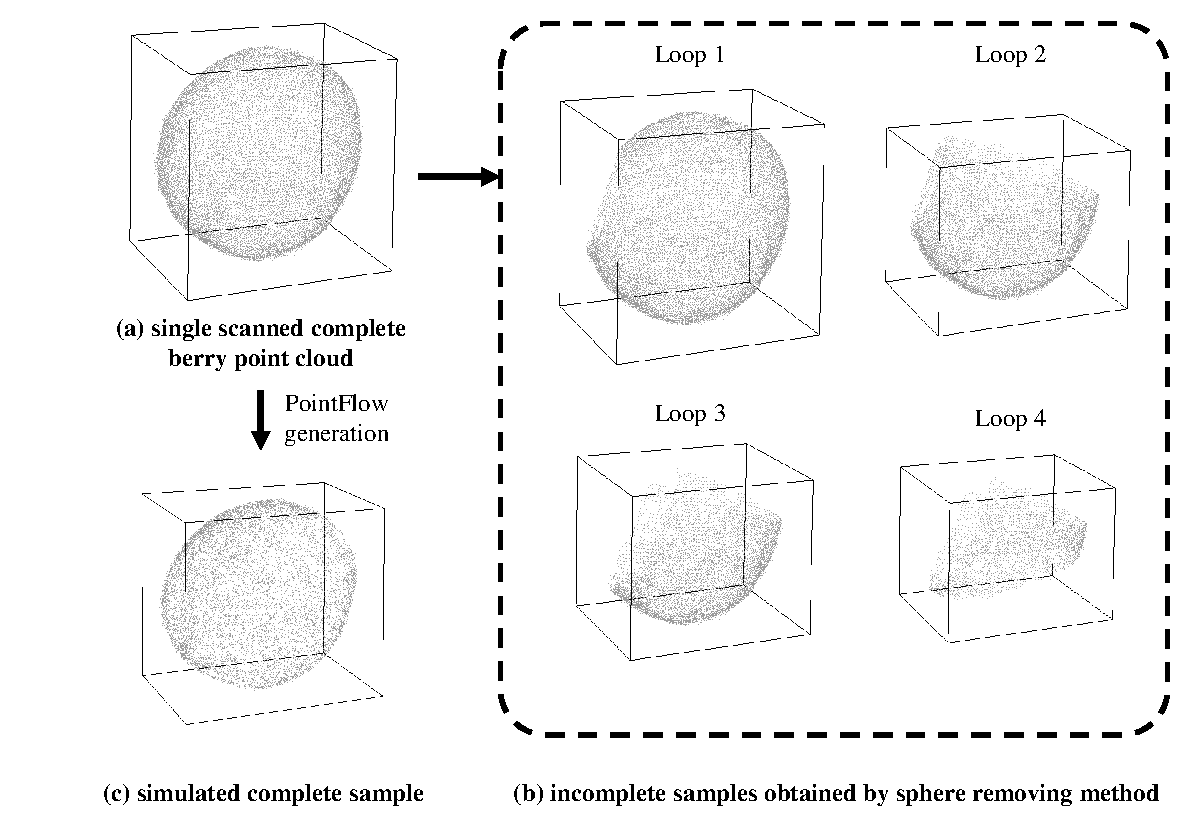
\includegraphics[width=1\textwidth]{figures/Figure9.pdf}
    \caption{\replaced[id=R2]{Workflow of automatic paired training dataset generation}{Example of dataset composition} for the \deleted[id=R2]{self-supervised training-based method of the} berry point cloud completion network.}
\end{figure}

%%%%%%%%%%%%%%%%%%%%%%%%%%%%%%%%%%%%%%%%%%%%%%%%%%%%%%%%%%%%%%%
\begin{reviewercomment}
    Table 3 results: Was the same dataset used to assess the other algorithms, or were those metrics taken from their original studies?
\end{reviewercomment}

\response{
    ...
}

\manuscript{
    ...
}


%%%%%%%%%%%%%%%%%%%%%%%%%%%%%%%%%%%%%%%%%%%%%%%%%%%%%%%%%%%%%%%
\begin{reviewercomment}
    Occlusion  threshold: Is there a berry-occlusion threshold? For example, if less  than 50\% of a berry is visible, is it included? How are barely visible  berries handled?
\end{reviewercomment}

\response{
    ...
}

\manuscript{
    ...
}


%%%%%%%%%%%%%%%%%%%%%%%%%%%%%%%%%%%%%%%%%%%%%%%%%%%%%%%%%%%%%%%
\begin{reviewercomment}
    Limitations \& future directions: How will the  model perform on wine grapes. Wine grapes accounts for ~60\% of US grape  production; clusters are denser, and berries are smaller than in table grapes.
\end{reviewercomment}

\response{
    ...
}

\manuscript{
    ...
}



\phantom{\cite{}} % 添加一个不可见的伪引用, 不会显示但能满足BibTeX要求避免无引用时报错
\bibliographystyle{elsarticle-harv}
\renewcommand{\bibsection}{} % 隐藏reference标题,如果需要则注释掉这一行
\bibliography{references}

\end{document}

% The copy-paste templates
\begin{verbatim}

    %%%%%%%%%%%%%%%%%%%%%%%%%%%%%%%%%%%%%%%%%%%%%%%%%%%%%%%%%%%%%%%
    \begin{reviewercomment}
        ...
    \end{reviewercomment}
    
    \response{
        ...
    }
    
    \manuscript{
        ...
    }
    
\end{verbatim}